\documentclass[12pt,parskip=full]{article}
\usepackage{lmodern}
\usepackage{amsmath}
\usepackage[left=1.0in,right=1.0in,top=0.5in,bottom=1.0in]{geometry}
\geometry{letterpaper}
\usepackage{graphicx}
\usepackage{caption}
\usepackage{subcaption}
\usepackage{longtable}
\usepackage{float}
\usepackage{wrapfig}
\usepackage{soul}
\usepackage{textcomp}
\usepackage{marvosym}
\usepackage{wasysym}
\usepackage{latexsym}
\usepackage{amssymb}
\usepackage{apacite}
\usepackage{tabu}
\usepackage[svgnames]{xcolor}
\usepackage{tikz}
\usepackage[linktoc=all]{hyperref}
\usepackage{cleveref}
\usepackage{listings}
\usepackage{setspace}
\usepackage{parskip}
\usepackage{array}
\usepackage{apacite}
\usepackage{natbib}
\usepackage{multicol}
\usepackage{subcaption}
\usepackage{mathtools}
\usetikzlibrary{arrows}

\pgfdeclarelayer{edgelayer}
\pgfdeclarelayer{nodelayer}
\pgfsetlayers{edgelayer,nodelayer,main}

\tikzstyle{none}=[inner sep=0pt]
\tikzstyle{waypt}=[circle,fill=Black,draw=Black,scale=0.4]
\tikzstyle{Helobody}=[circle,fill=White,draw=Black,scale=4.0]
\tikzstyle{Tailrotor}=[circle,fill=White,draw=Black,scale=1.0]
\tikzstyle{ForceVector}=[->,draw=Indigo,fill=Indigo]
\tikzstyle{Coordinate}=[->,draw=Red,fill=Red,fill opacity=1.0]
\tikzstyle{angle}=[->]
\tikzstyle{MeasureMark}=[|-|]
\newlength{\imagewidth}
\newlength{\imagescale}

\setlength{\parskip}{11pt}
%\setlength{\parindent}{15pt}
\usepackage{bookmark}
\makeatletter
\renewcommand\@seccntformat[1]{}
\makeatother

\lstset
{
    language=c,
    keywords={break,case,catch,continue,else,for,
        if,return,switch,try,while,int,void},
    basicstyle=\ttfamily,
    keywordstyle=\color{blue},
    commentstyle=\color{ForestGreen},
    stringstyle=\color{purple},
    numbers=left,
    numberstyle=\tiny\color{gray},
    stepnumber=1,
    numbersep=10pt,
    backgroundcolor=\color{white},
    tabsize=4,
    showspaces=false,
    showstringspaces=false
}

\renewcommand{\thesection}{\arabic{section}}

\renewcommand{\thesubsection}{\thesection\alph{subsection}}
\renewcommand{\theequation}{\thesubsection\arabic{equation}}
\newcommand*\circled[1]{\tikz[baseline=(char.base)]{
            \node[shape=circle,draw,inner sep=1pt] (char) {#1};}}
            
\numberwithin{subsection}{section}

\begin{document}
	\vspace{-4ex}
	\title{Final Project\vspace{-3.5ex}}
	\author{Rob Rau\vspace{-4ex}}
	\date{\today\vspace{-4ex}}
	\maketitle

	\section{Introduction}
		For this term project I impliment parallelization of my own computational fluid dynamics (CFD) software and I explore load balancing
		for heterogenous compute networks. In this report I will discuss how I parallelized my code, scaling results, my method of
		load balancing, and present results for both simulated heterogenous networks and a real heterogenous network. 

	\section{CFD}
		The first step the needed to be completed in this project was to parallelize my computational fluid dynamics code, EbbCFD.
		EbbCFD is a 2 dimensional second order finite volume code that currently only solves the Euler equations. It operates on a
		mesh consisting of triangles, where each triangle represents a finite volume (or area in 2D) that we use to approximate the
		solution state in. A finite volume code works by computing the flux between two cells and using those fluxes to update the
		average solution state of the cells. For triangular meshes, each cells will have 3 flux values that are used to compute the
		current solution state. A first order code will use the cell averaged values to compute the fluxes between two cells, where
		as a second order code will compute an approximation of the solution state gradient, use said gradient to compute the solution
		state at the cell edges, and use those edge values to compute the flux.
		
		% make clear with a few formulas

		To parallelize this sort of code, I (and most other people) divide up the mesh into sub-meshes that each processor then computes.
		This means that each processor will need to communicate information to processors that are geometrically next to them on the 
		mesh. This means that for a first order code, the cell averaged solution state of the outer edge of the submesh will need to be
		sent to the relevant neighbors each timestep. A second order code is a bit more tricky. The cell averaged solution state still
		needs to be communicated but as there are now gradients and edge state values, we need to send more information. I broke down my
		commuication into two steps: an average state update, and an edge state update. Each processor maintains extra cells around its
		submesh that represent the relevent cells of its neighbors, typically called halo cells. In the first communication step these
		cells are populated with average state information. That information is then used to compute gradients and edge values. The
		second communication step then sends the computed edge values so neighbor processors can compute the necessary fluxes.
		This constitutes the bulk of the communication that needs to happen, but it doesn't account for all. 
		% show partitioned mesh

		\begin{figure}[H]
			\centering
			\begin{subfigure}[H]{0.6\textwidth}
				\makebox[\textwidth]{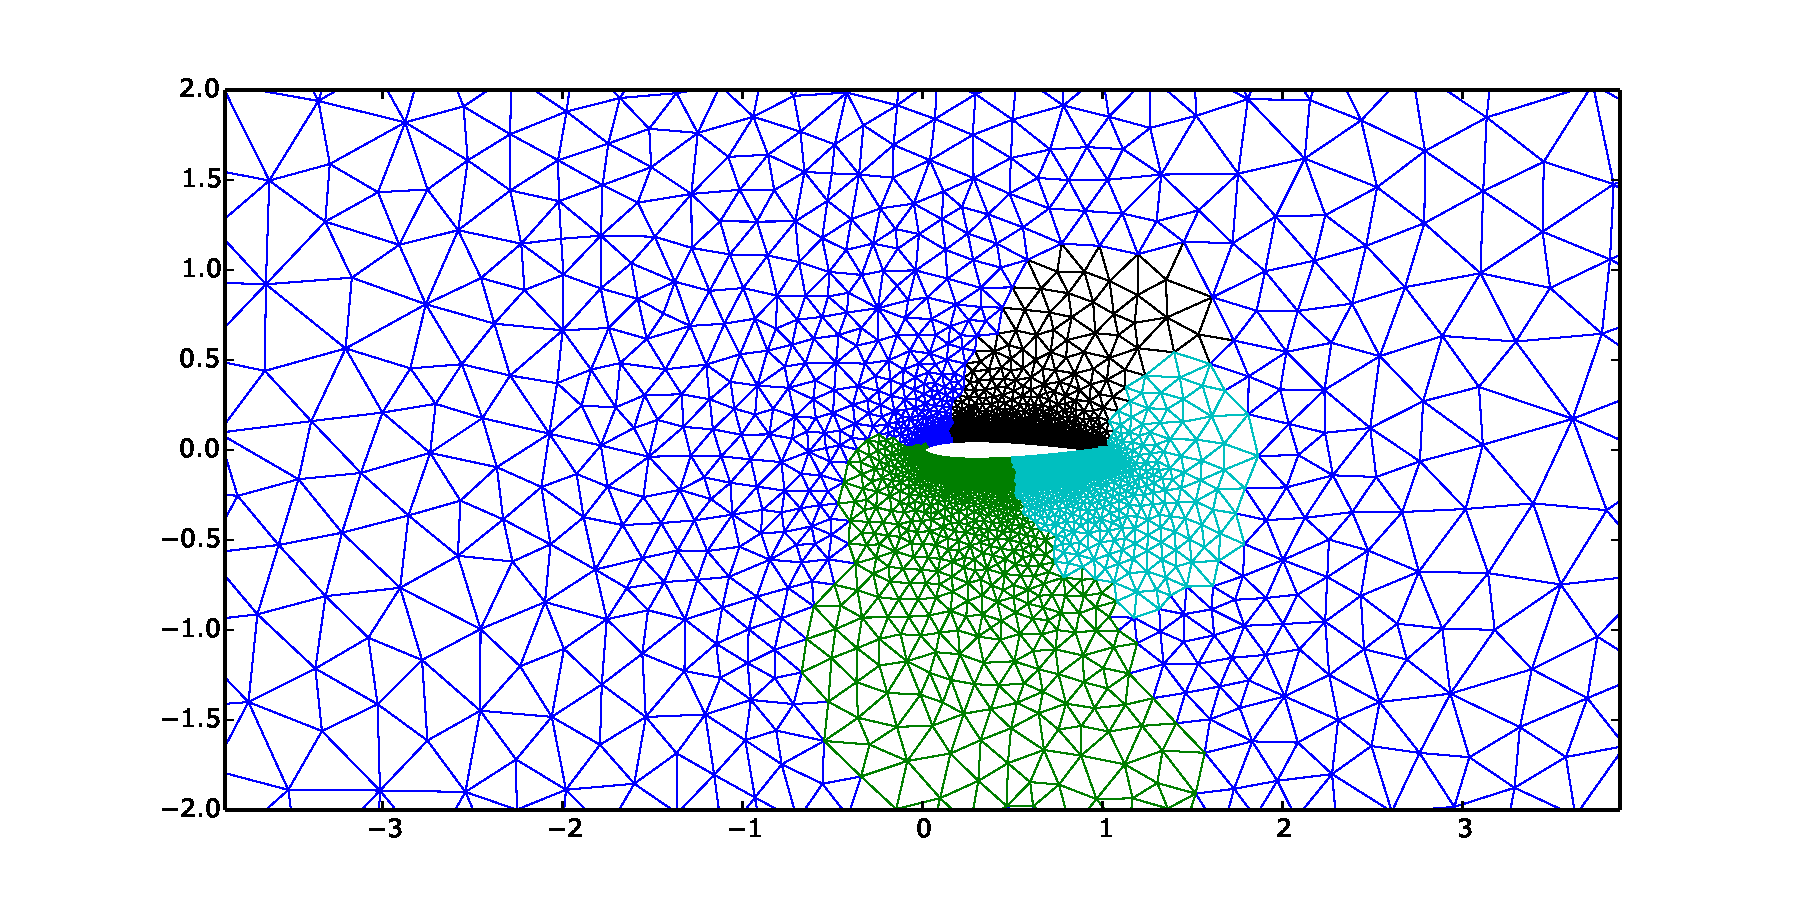
\includegraphics[width=2\textwidth]{Meshes.pdf}}
			\end{subfigure}
			\begin{subfigure}[H]{0.6\textwidth}
				\makebox[\textwidth]{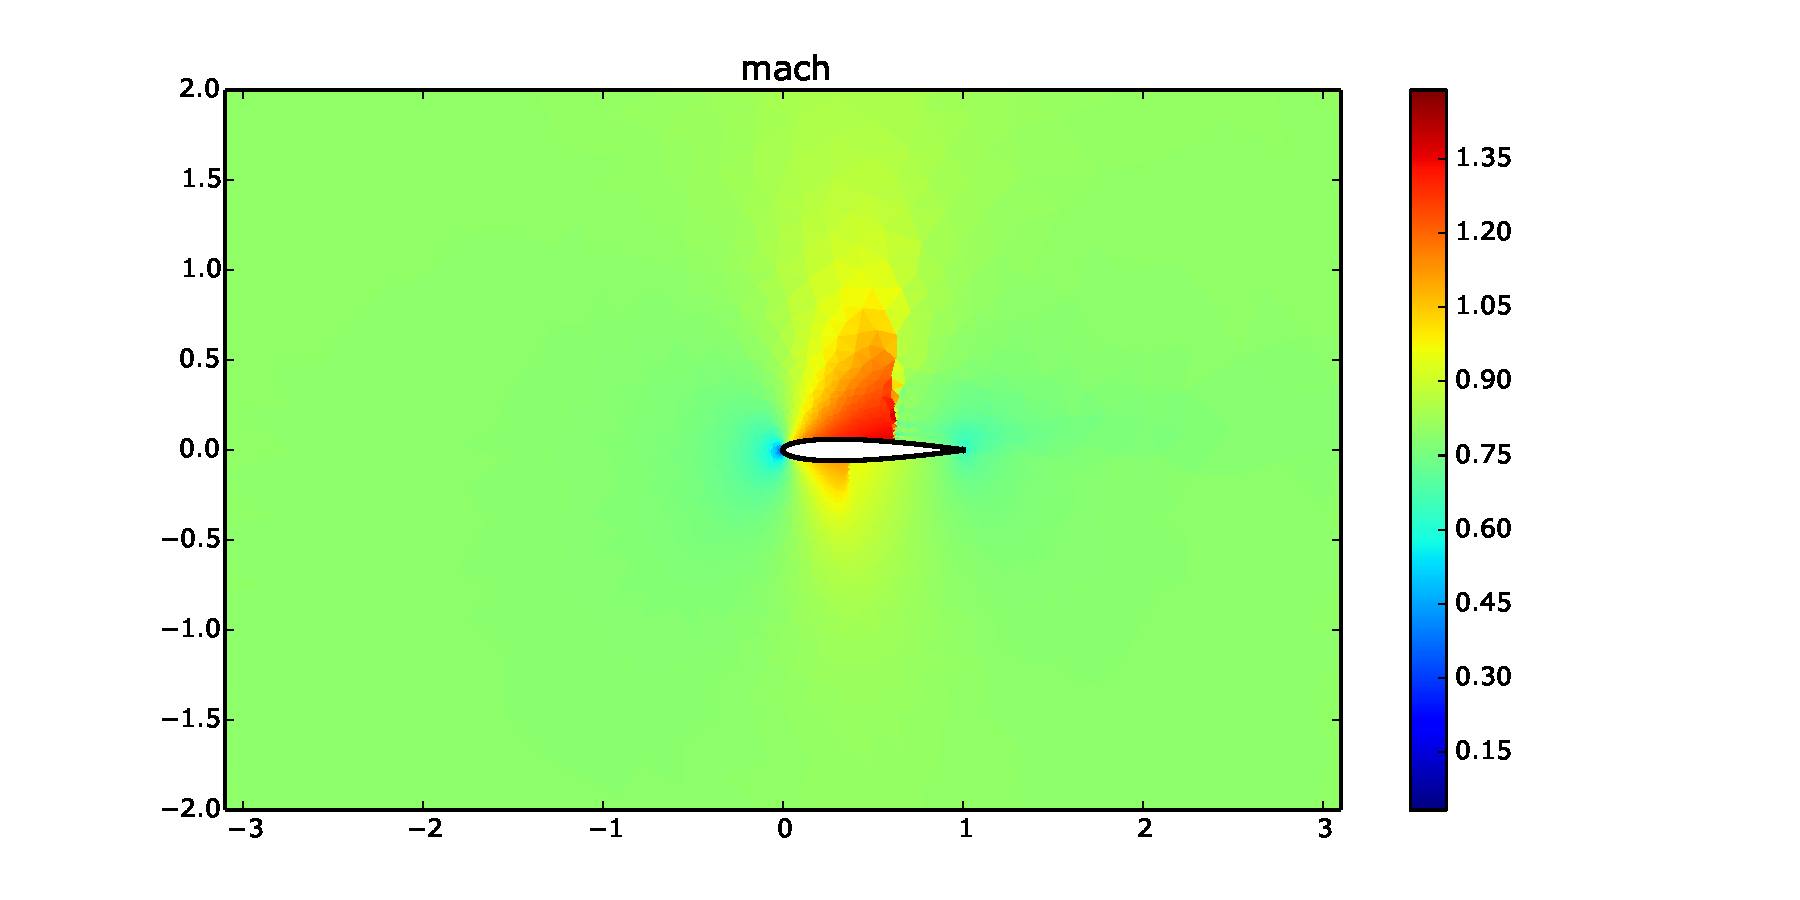
\includegraphics[width=2\textwidth]{EbbSolution.pdf}}
			\end{subfigure}
		\end{figure}
		There are other things, not directly tied to the solution that need to be communicated to considered a fully featured code.
		CFD codes need to be able to compute forces imparted by the flow onto solid boundaries, they need to compute solution residuals,
		and they often will dynamically set the timestep based off the solution. All of these things come down to performing reduce
		operations every timestep. Overall this is relativly easy but still something that needs to be considered.

		To reduce the overhead of the two comunication steps in the core of my solver, I resorted to using non blocking communications,
		which CFD lends itself to relativly well. Typically only a small portion of what needs to be computed relies on communicated data.
		So to address this, sends and receives are started with \verb|MPI_Startall|, work is done on other parts of the mesh, and when we
		need the data, we block until \verb|MPI_Testall| tells us that our communications have arrived. Switching to this method improved scaling
		on high latency networks like ethernet.
		% show those scalling results 

		EbbCFD scaled fairly well to ~200 elements per processor. I tested both a ~6400 element mesh and a ~11000 element mesh. The following
		plot shows that with more elements, more processors are more effective, indicating communication overhead being the
		bottle neck. Of course this makes sense, the fewer elements per processor, the less time it takes to compute those elements,
		and communication time takes a higher percentage of the total iteration time. Non-blocking communications helps with this
		some, but there always becomes a point where more processors are no longer effective. 
		
		\begin{figure}[H]
			\centering
			\begin{subfigure}[H]{0.3\textwidth}
				\makebox[0cm]{\includegraphics[width=1.8\textwidth]{EbbSpeedup.pdf}}
			\end{subfigure}
			\begin{subfigure}[H]{0.3\textwidth}
				\makebox[9cm]{\includegraphics[width=1.8\textwidth]{EbbEfficiency.pdf}}
			\end{subfigure}
		\end{figure}

	\section{Optimization}
		My approach to load balancing was through mathmatical optimization. Basically solving the following problem
		\begin{align}
			\mathrm{minimize \ }& f(x) \\
			\mathrm{subject \ to \ } & c_j(x) = 0, \quad c_k(x) >= 0
		\end{align}
		where $f(x)$ is the average computational time for one timestep of the simulation and $c_j(x)$ are the equality constraints and 
		$c_k(x)$ are the inequality constraints. The constraints for this problem are determined by metis, the mesh partition library used.
		Metis requires that each weight satisfy $0 \le w_i \le 1$ and that
		\begin{equation}
			0 = 1 - \sum{w_i} \quad i = 1,..,p
		\end{equation}
		
		The thing with mathmatical optimization is that it assumes smooth continuous functions. The thing with computers is that they
		typically aren't smooth continouos devices. Interestingly enough, for this problem at least, this can be spoofed to be the case.
		I found that by taking long enough runtime samples of my code, the average iteration time, measured in seconds, stayed stable.
		Typically to about 4 significant figures. This, coupled with the fact that, for a two dimensional mesh, computation time scales
		as expected with $O(N^2)$, we have a potential recipe for mathmatical optimization. 
		% talk about mathmatical optimization

		There are many different algorithms that solve optimization problems, but most fall into two catagories: gradient based optimization,
		and gradient free optimization. Gradient free approaches vary wildly in their fundamental concepts. Genetic algorithms in a way
		attempt to emulate evolution, simplex methods compute the objective function at the points of an $n + 1$ dimensional simplex, and
		find search directions using that, and the partical swarm optimizer emulates particles in a feild, traveling towards a minimum point.
		In my past research with various optimization methods, I typically found that gradient free approaches, while work, usually converge
		slower, and can require more computations of the objective function that their gradient based counterparts.

		For this reason I decided to use a quasi-newton gradient based optimizer. In gradient based optimization, the gradient of the objective
		function $\nabla f(x)$ needs to be know as well as the Hessian matrix, defined by
		\begin{equation}
			\nabla^2 f(x) = H(x) = \begin{bmatrix}
				\frac{\partial^2 f}{\partial^2 x_1} & \dots & \frac{\partial^2 f}{\partial x_1 \partial x_n} \\
				\vdots & \ddots & \vdots \\
				\frac{\partial^2 f}{\partial x_n \partial x_1} & \dots & \frac{\partial^2 f}{\partial^2 x_n}
			\end{bmatrix}
		\end{equation}

		Unfortunatly the gradient needs to be computed at each $x$ visited. However, using the quasi-newton method BFGS (Broyden-Fletcher-Goldfarb-Shanno),
		the Hessian matrix is is not computed at each iteration, but it is estimated and updated as the optimizer moves through the design space. This saves
		us from needing to compute $n^2$ second derivatives, and only computing $n$ derivatives. Using a central difference scheme, this ends up 
		computing the objective function $2n + 1$ times per iteration. The BFGS method is formulated for unconstrained optimization, but we clearly
		have constraints that need to satisfied, so in comes Sequentail Quadratic Programming (SQP). SQP is a modification on top of BFGS to
		allow for equality constraints, that basically solves the problem
		\begin{equation}
			\mathrm{minimize} \phi(x) = f(x) + \frac{1}{\mu}||c||_1
		\end{equation}
		where
		\begin{equation}
			||c||_1 = \sum{|c_j|}
		\end{equation}

		Metis requires us to have inequality constraints as well. Fortunatly a relatively minor modification can be made to SQP to allow for this.
		It becomes what we call an active set method. Basically every iteration we test where the solution is and where it want't to go and
		update inequality constraints to equality constraints if they are going to be violated.

		Computing the gradient at every iteration may at first seem like a lot of overhead, but I implimented the code so that solution always marches
		forward, even at the intermediate mesh weights. This required keeping the un partitioned mesh on processor 0 and scattering and gathering
		results to and from the partitioned mesh. While this does add overhead, it ensures, that while an optimal mesh partition may not yet be acheived
		actual work is still being done. As shown later, the optimizer never strays far from optimality so the runtime never gets significantly worse.
		
		For the finite difference derivative approximation, I found that setting the step size to $h = \frac{300}{N}$ provided reasonable results.
		It ensured that enough cells where removed or added to make an appreciable difference in compute time.

	\section{Results}
		To test this method, I artificially slowed down some processors and let the optimizer run. To simulate network configuration changes, I could
		change which processors were slowed down. This allowed for isolated testing in an enviroment like Flux, with low latency/high bandwidth interconnects.
		I also tested on a live ethernet network between computers of varying capabilities without any artificial slowdowns.

		Running on Flux, without simulating a network change, it the optimizer finds its way to an optimal mesh distribution in relatively few iterations,
		yeilding a \% increase in computation speed.
		% put figures here and also proper numbers


		The following results come from a simulated network change. The code monitors the running time of the core solver and if it detects a significant
		change in run time, it will trigger the optimizer to run again. Whether the optimizer starts at an even mesh distribution or the last optimal mesh
		distribution is a question of scenario. If a wildly different configuration happens, like what is simulated, I found it's better to restart
		the optimizer with equal weights. If the change is less extreme it can be beneficial to start with the old optimal solution with the hopes
		that the new optimal point is not far away. Either way, it can be seen that it detects the change, and re-balances to the optimal point.
		\begin{figure}[H]
			\centering
			\begin{subfigure}[H]{0.9\textwidth}
				\includegraphics[width=\textwidth]{5PnetworkChange.pdf}
				\caption{Network configuration change restarting with equal mesh partitions}
			\end{subfigure}
			\begin{subfigure}[H]{0.9\textwidth}
				\includegraphics[width=\textwidth]{6PNetworkChange.pdf}
				\caption{Network configuration change restarting with previous best mesh partitions}
			\end{subfigure}
		\end{figure}
		% insert network change plots

		For the following test, I ran this on my home gigabit ethernet network on the following machines.

		\begin{centering}
		\begin{tabular}{| m{1.8cm} | m{1.5cm} | c | c | m{1.5cm} | m{2cm} | m{1.8cm} | m{2cm} | }
			\hline
			Machine &	              L1 D/I cache & L2 cache & L3 cache & CPU &	    Operating frequency & CPUS(hw threads) & RAM \\ \hline\hline
			2011 MacBook Pro 	    & 32k/32k      & 256k     & 6144k    & Intel I7-2720MQ & 2200Mhz & 4(8) & 16GB DDR3 1333Mhz \\ \hline
			2015 Dell Precision M6800   & 32k/32k	   & 256k     & 8192k    & Intel I7-4910MQ & 2900Mhz & 4(8) & 32GB DDR3 1600Mhz \\ \hline
			2012 Custom Desktop	    & 32k/32k	   & 256k     & 8192k	 & Intel I7-2600K  & 3400Mhz & 4(8) & 16GB DDR3 1867Mhz \\ \hline
		\end{tabular}
		\end{centering}

		The following results where from a 6 processor run, with each machine running 2 processors. Even on a high latency/low bandwidth (relative to 
		InfinaBand) network the optimizer managed to distribute the mesh in a way one would expect, and yeild a \% increas in computation speed.
		\begin{figure}[H]
			\centering
			\begin{subfigure}[H]{0.9\textwidth}
				\includegraphics[width=\textwidth]{RealNetwork.pdf}
				\caption{6 processors on a quiet ethernet network with no other computational activity}
			\end{subfigure}
			\begin{subfigure}[H]{0.9\textwidth}
				\includegraphics[width=\textwidth]{RealNetwork2.pdf}
				\caption{6 processors on a less quiet ethernet network with various other computational activity}
			\end{subfigure}
		\end{figure}
		% put figure in here and also proper numbers

		% show plots of mesh weights vs time (optimization iteration)
		% show plots of average iteration time vs time (optimization iteration)


	\section{Conclusions}

		The overall concept did yeild positive results and for the cases I tested, a speedup was acheived in both more isolated environment like flux
		and in a noisy live environment like my livingroom. 
		% talk about benefits

		In the testing I carried out I could not get appreciable speedup above 6 processors and unfortunatly I don't have a good explination for why.
		Perhaps a different underlying optimization algorithm could fix this. 
		% talk about limitations
		
		There are two primary applications that I see this approach being useful: small beowolf clusters, and CPU/GPU hybrid code. There are many people
		who don't have access to large HPC compute resources, but do have many machines laying around capable of being used. My living room being a prime
		example. Once I graduate, I will won't have as readily available access to Flux, but I have other machines I can use to compute in parallel. As I
		continue to develope EbbCFD and add in expensive viscouse flux calculations and add 3D support have this option open to me is a huge boon. I also
		have many graphics cards available to me as an avid gamer, and I can see this approach working to balance CPU/GPU code execution on large enough
		data sets.

		All code relevent to this project is up on Github at the following URL's: \url{https://github.com/Rob-Rau/EbbCFD} and \url{https://github.com/Rob-Rau/numd}.
		The numd repository contains the code for the optimizer. The specific file is \verb|numd/optimization/SQP.d|
	\section{Future Work}
		Even though I am a masters student I do have plans to extend this. The two main things I'm currently interested in are, as mentioned above, CPU/GPU
		balancing, and testing different optimization algorithms. I'd like to test some gradient free methods, most likely simplex methods, and see if I
		can acheive better scaling results. 
		% talk about possible real world applications (GPU/CPU balancing)


\end{document}
